\documentclass[12pt]{article}
% Full article preamble (duplicated, no common file)
\usepackage{fontspec}
\usepackage[a4paper,margin=2.5cm,includefoot]{geometry}
\usepackage{polyglossia}
\usepackage{amsmath}
\usepackage{amssymb}
\usepackage{xcolor}
\usepackage{fancyhdr}
\usepackage{graphicx}
\usepackage{listings}
\usepackage[most]{tcolorbox}
\usepackage{pifont}
\usepackage{enumitem}
\usepackage{titlesec}
\usepackage[bottom]{footmisc}
\usepackage{titling}
\usepackage{minted}
\usepackage{etoolbox}
\usepackage{array}
\usepackage{extsizes}

\newfontfamily\emoji{Segoe UI Emoji}

\pagestyle{fancy}

\setmainlanguage[numerals=western]{arabic}
\setotherlanguage{english}
\newfontfamily\arabicfont[Script=Arabic]{Amiri}
\newfontfamily\arabicfonttt[Script=Arabic]{Courier New}

\lstset{
  language=[Sharp]C,
  numbers=left,
  stepnumber=1,
  numbersep=8pt,
  frame=single,
  basicstyle=\ttfamily\small,
  keywordstyle=\color{blue},
  stringstyle=\color{red},
  commentstyle=\color{green!50!black}
}

\newif\ifdetailed
\ifdefined\setdetailed
  \setdetailed
\fi

\newif\ifwithsols
\ifdefined\setwithsols
  \setwithsols
\fi

% unified tcolorboxes for articles
\tcbset{colback=white, colframe=black, fonttitle=\bfseries, boxrule=0.8pt}
\newtcolorbox{boxDef}[1][]{colback=blue!5!white,colframe=blue!75!black,
  title={{\emoji📘} تعريف\ifx\\#1\\\else ~#1\fi :}}
\newtcolorbox{boxExercise}[1][]{colback=cyan!5!white,colframe=cyan!70!black,
  title={{\emoji🧩} تمرين\ifx\\#1\\\else ~#1\fi :}}
\newtcolorbox{boxExample}[1][]{colback=yellow!5!white,colframe=orange!90!black,
  title={{\emoji📝} مثال\ifx\\#1\\\else ~#1\fi :}}
\newtcolorbox{boxNote}[1][]{colback=gray!10!white,colframe=black,
  title={{\emoji✨} ملاحظة\ifx\\#1\\\else ~#1\fi :}}
\newtcolorbox{boxAttention}[1][]{colback=magenta!10!white,colframe=magenta!80!black,
  title={{\emoji🔔} تنبيه\ifx\\#1\\\else ~#1\fi :}}
\newtcolorbox{boxWarning}[1][]{colback=red!5!white,colframe=red!75!black,
  title={{\emoji⚡} ملاحظة هامة\ifx\\#1\\\else ~#1\fi :}}
\newtcolorbox{boxSolution}[1][]{colback=green!5!white,colframe=green!60!black,
  title={{\emoji✅} حل\ifx\\#1\\\else ~#1\fi :}}
\newtcolorbox{boxSymbol}[1][]{colback=purple!5!white,colframe=purple!70!black,
  title={{\emoji🔣} رمز\ifx\\#1\\\else ~#1\fi :}}

\tcbset{simplecode/.style={ colback=gray!5, colframe=black!50, boxrule=0.4pt, arc=2pt, left=4pt,right=4pt,top=4pt,bottom=4pt}}
\newenvironment{boxCode}{\begin{tcolorbox}[simplecode]}{\end{tcolorbox}}

\newcolumntype{C}[1]{>{\centering\arraybackslash}p{#1}}

% redefine spaces after titles
\makeatletter
\renewcommand{\@maketitle}{%
  \begin{center}
    {\huge \bfseries \@title \par}%
    \vskip 0.2em % space between title and author
    {\large \@author \par}%
    % \vskip 0.2em % space between author and date
    % {\normalsize \@date \par}%
  \end{center}
}
\makeatother

\fancyhf{} % clear default
\fancypagestyle{plain}{
  \fancyhf{}
  \fancyhead[L]{مدرسة التسامح الشاملة}
  % \fancyhead[L]{
\includegraphics[height=1cm]{../../../images/logoTasamoh.png}}
  \fancyhead[R]{الأستاذ محمود اغبارية}
  \fancyfoot[C]{\thepage}
}

\fancyhead[L]{مدرسة التسامح الشاملة}
\fancyhead[R]{الأستاذ محمود اغبارية}
\fancyfoot[C]{\thepage}
% \date{\today}

\setcounter{tocdepth}{3} % only section subsection and subsubsection in TOC


% ----------------------


% \begin{document}

% \maketitle

% % \clearpage  % start TOC on a new page
% % \renewcommand{\contentsname}{جدول المحتويات}
% % \tableofcontents
% % \clearpage

% \part*{part 1} % the * prevents numbering
% \section*{مقدمة}
% \subsection*{مثال رياضي}
% \subsubsection*{مثال فرعي}
% \paragraph*{ paragraph 1}
% \subparagraph*{sub paragraph 1}

% \ifdetailed
% \begin{english}
% \begin{minted}{csharp}
% // C# Example
% \end{minted}
% \end{english}
% \fi

% OLD WAY
% \ifdetailed
% \begin{english}
% \begin{lstlisting}
% // C# Example
% \end{lstlisting}
% \end{english}
% \fi

% % 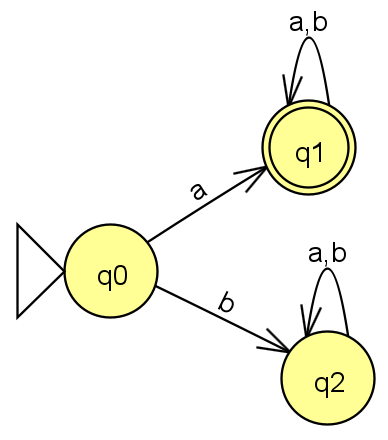
\includegraphics[width=0.2\textwidth]{../../../images/DFAs/ex1_q1.png}



% \vspace{3cm}
% \begin{flushleft}
% أرجو لكم وقتًا ممتعًا.

% الأستاذ محمود اغبارية.
% \end{flushleft}


% \end{document}


\title{العمليات الخارجية في لغة \textenglish{C\#} }

\begin{document}
\maketitle

\section*{مقدمة}
العمليات هي وسيلة لتقسيم البرنامج إلى مقاطع صغيرة تؤدي مهام محددة.
تساعد العمليات على:
\begin{itemize}
    \item تنظيم الكود وجعله أسهل للقراءة والصيانة.
    \item إعادة استخدام نفس الكود أكثر من مرة.
\end{itemize}

في هذا الدرس سنتعرّف على أنواع العمليات من حيث استقبال المعطيات (البارامترات) وإرجاع القيم، وكيف نعرّفها داخل الصف.

\section{مبنى تعريف العملية}
كل عملية في لغة C\# تتكوّن من قسمين رئيسيين:

\begin{enumerate}
    \item \textbf{تعريف العملية} \textenglish{(Method Signature)}
    وهي السطر الأول الذي يحتوي على:
    \begin{itemize}
        \item نوع العملية، في هذه المرحلة دائمًا سوف نستعمل: \textenglish{public static}
        \item نوع القيمة التي تعيدها (\textenglish{void, int, double, bool, string, char})
        \item اسم العملية. ومن المتبع أنّ اسم العملية يبدأ دائمًا بحرف كبير
        \item البارامترات بين الأقواس (مثل \textenglish{(int x, int y)})
    \end{itemize}

    \item \textbf{جسم العملية} \textenglish{(Function Body)}
    وهو الكود الموجود بين القوسين \textenglish{\{ \}}، ويحتوي على التعليمات التي تُنفّذ عند استدعاء العملية.
\end{enumerate}

\begin{boxExample}[1]
\begin{english}
\begin{minted}{csharp}
public static void PrintHello()
{
    Console.WriteLine("Hello");
}
\end{minted}
\end{english}
\hrule
\begin{itemize}
    \item \textenglish{public static} $\leftarrow$ جزء ثابت.
    \item \textenglish{void} $\leftarrow$ العملية لا ترجع شيئًا.
    \item \textenglish{PrintHello} $\leftarrow$ اسم العملية.
    \item \textenglish{()} $\leftarrow$ الأقواس الفارغة بعد اسم العملية معناها أنّ هذه العملية لا تستقبل بارامترات.
    \item ما بين الأقواس \textenglish{\{ \}} هو جسم العملية، وفي هذه الحالة يطبع رسالة \textenglish{Hello}.
\end{itemize}
\end{boxExample}

\begin{boxExample}[2]
\begin{english}
\begin{minted}{csharp}
public static int AddNumbers(int a, int b)
{
    int sum = a + b;
    return sum;
}
\end{minted}
\end{english}
\hrule
\begin{itemize}
    \item \textenglish{public static} $\leftarrow$ جزء ثابت.
    \item \textenglish{int} $\leftarrow$ نوع القيمة المرجعة.
    \item \textenglish{AddNumbers} $\leftarrow$ اسم العملية.
    \item \textenglish{(int a, int b)} $\leftarrow$ البارامترات التي تستقبلها العملية، في هذه الحالة تستقبل متغيرين كلاهما من نمط \textenglish{int}.
    \item ما بين الأقواس \textenglish{\{ \}} هو جسم العملية، الذي ينفّذ عملية الجمع ويعيد النتيجة.
    \item نستخدم كلمة \textenglish{return} لننهي العملية ونعيد القيمة المطلوبة. \\
    \textbf{ملاحظة:} نوع القيمة التي ترجعها العملية يجب أن يطابق نوع القيمة بعد كلمة \textenglish{return}.
\end{itemize}
\end{boxExample}

\section{استدعاء العملية}
بشكل عام، لكي نستدعي عملية خارجية نكتب اسم الفئة، ثم نقطة ثم اسم العملية.

في البداية سوف نتعامل مع عمليات معرفة داخل الفئة التي نعمل فيها \textenglish{Program}. \\
في هذه الحالة لا حاجة لكتابة اسم الفئة، نكتب فقط اسم العملية.

مثلًا، لكي نستدعي العمليتين اللتين عرفناهما أعلاه:

\begin{boxExample}
\begin{english}
\begin{minted}{csharp}
public static void Main(string[] args)
{
    PrintHello();
    int sum1 = AddNumbers(5, 10);
    int a = 5;
    int b = 10;
    int sum2 = AddNumbers(a, b);
}
\end{minted}
\end{english}
\end{boxExample}


\begin{itemize}
    \item العملية \textenglish{PrintHello()} لا ترجع أي قيمة، لذلك لم نحتج أن نحفظها في متغير.
    \item العملية \textenglish{AddNumbers(int a, int b)} ترجع قيمة، لذلك نحفظها في متغير \textenglish{sum}.
    \item المتغير الذي نحفظ فيه قيمة العملية يجب أن يكون من نفس النوع الذي ترجعه العملية.
    \item البارامترات التي نعطيها للعملية يجب أن تكون من نفس النوع الموجود في تعريف العملية وبنفس الترتيب.
\end{itemize}

\subsection*{استدعاء عملية من فئة أخرى}
كما ذكرنا أعلاه، في هذه الحالة علينا أن نكتب اسم الفئة، ثم نقطة ثم اسم العملية. \\
نحن نعرف الكثير من هذه العمليات:
\begin{itemize}
    \item \textenglish{Console.WriteLine("Hello World!");} \\
    هذا استدعاء للعملية \textenglish{WriteLine} من الفئة \textenglish{Console}
    \item \textenglish{Console.ReadLine();} \\
    هذا استدعاء للعملية \textenglish{ReadLine} من الفئة \textenglish{Console}
    \item \textenglish{Math.Max(5, 10);} \\
    هذا استدعاء للعملية \textenglish{Max} من الفئة \textenglish{Math}
    \item \textenglish{Math.Min(5, 10);} \\
    هذا استدعاء للعملية \textenglish{Min} من الفئة \textenglish{Math}
    \item \textenglish{Math.Abs(-5); } \\
    هذا استدعاء للعملية \textenglish{Abs} من الفئة \textenglish{Math}
    \item \textenglish{Math.Pow(2, 3); } \\
    هذا استدعاء للعملية \textenglish{Pow} من الفئة \textenglish{Math}
    \item \textenglish{Math.Sqrt(25); } \\
    هذا استدعاء للعملية \textenglish{Sqrt} من الفئة \textenglish{Math}
    \item \textenglish{Math.Round(2.5); } \\
    هذا استدعاء للعملية \textenglish{Round} من الفئة \textenglish{Math}
\end{itemize}

\clearpage
\section{أنواع العمليات}

\subsection{لا ترجع ولا تستقبل بارامترات}
نستخدمها عندما نريد تنفيذ أمر محدد دون الحاجة لإدخال أو إخراج بيانات.

\begin{boxExample}
\begin{english}
\begin{minted}{csharp}
public static void PrintWelcome()
{
    Console.WriteLine("Welcome to the program!");
}

public static void Main()
{
    PrintWelcome();
}
\end{minted}
\end{english}
\end{boxExample}

عملية بسيطة تطبع رسالة فقط. لا تحتاج لأي معطيات ولا ترجع أي نتيجة.

\subsection{تستقبل ولا ترجع}
تستقبل معطيات (parameters) لكنها لا تعيد قيمة.

\begin{boxExample}[1]
\begin{english}
\begin{minted}{csharp}
public static void PrintSum(int a, int b)
{
    int sum = a + b;
    Console.WriteLine("Sum = " + sum);
}

public static void Main()
{
    PrintSum(5, 3);
}
\end{minted}
\end{english}
\end{boxExample}

العملية تستقبل عددين وتطبع ناتج جمعهما فقط، دون إرجاع النتيجة. \\

يمكننا أيضًا استخدام متغيرات كبرامترات عند استدعاء العملية:
\begin{boxExample}[2]
\begin{english}
\begin{minted}{csharp}
public static void PrintSum(int a, int b)
{
    int sum = a + b;
    Console.WriteLine("Sum = " + sum);
}

public static void Main()
{
    int x = 5;
    int y = 3;
    PrintSum(x, y);
}
\end{minted}
\end{english}
\end{boxExample}

\textbf{مثال لعملية كهذه نعرفها:} \\
\textenglish{Console.WriteLine()} \\
هي عملية تستقبل بارامتر واحد من نمط \textenglish{string} ولا تعيد أي قيمة. \\
بما أنّ هذه العملية معرّفة في فئة أخرى غير، فعلينا كتابة اسم الفئة في هذه الحالة \textenglish{Console}.

\subsection{ترجع ولا تستقبل}
تقوم بإرجاع نتيجة معينة دون الحاجة لمعطيات.

\begin{boxExample}
\begin{english}
\begin{minted}{csharp}
public static int ReadNumber()
{
    int num = int.Parse(Console.ReadLine());
    return num;
}

public static void Main()
{
    int x = ReadNumber();
    Console.WriteLine("The number: " + x);
}
\end{minted}
\end{english}
\end{boxExample}

العملية لا تحتاج مدخلات، لكنها ترجع عددًا يمكننا استخدامه في البرنامج.

\textbf{مثال لعملية كهذه نعرفها:} \\
\textenglish{Console.ReadLine()} \\
هي عملية لا تستقبل أي بارامتر، لكنها تعيد قيمة من نمط \textenglish{string}. \\
بما أنّ هذه العملية معرّفة في فئة أخرى غير، فعلينا كتابة اسم الفئة في هذه الحالة \textenglish{Console}.

\subsection{تستقبل وترجع}
تستقبل معطيات وتعيد ناتجًا جديدًا بعد معالجتها.

\begin{boxExample}
\begin{english}
\begin{minted}{csharp}
public static double GetAverage(double a, double b)
{
    double avg = (a + b) / 2.0;
    return avg;
}

public static void Main()
{
    double result = GetAverage(7.5, 9.0);
    Console.WriteLine("Average = " + result);
}
\end{minted}
\end{english}
\end{boxExample}

العملية تستقبل عددين وتحسب معدلهما ثم تعيد النتيجة.

\subsection*{أمثلة نعرفها}
\begin{itemize}
    \item \textenglish{Math.Max} و \textenglish{Math.Min} هما عمليتان تستقبل كل واحدة منهما عددين من نمط \textenglish{int} وترجع قيمة من نمط \textenglish{int}.
    \item \textenglish{Math.Abs} و \textenglish{Math.Pow} هما عمليتان تستقبل كل واحدة منهما عددين من نمط \textenglish{double} وترجع قيمة من نمط \textenglish{double}.
    \item \textenglish{Math.Round} و \textenglish{Math.Sqrt} هما عمليتان تستقبل كل واحدة منهما عددًا من نمط \textenglish{double} وترجع قيمة من نمط \textenglish{double}.
    \item \textenglish{int.Parse} هي عملية تستقبل بارامترًا واحدًا من نمط \textenglish{string} وترجع قيمة من نمط \textenglish{int}.
    \item \textenglish{double.Parse} هي عملية تستقبل بارامترًا واحدًا من نمط \textenglish{string} وترجع قيمة من نمط \textenglish{double}.
\end{itemize}

\section{ملاحظات مهمة}

\begin{itemize}
\item
    يُفضّل أن يبدأ اسم العملية بحرف كبير وأن يصف وظيفتها بوضوح. \\
وإذا كان اسمها مكونًا من أكثر من كلمة، فكل كلمة تبدأ بحرف كبير
\begin{itemize}
    \item \textenglish{CalculateSum()}
    \item \textenglish{GetMaxValue()}
    \item \textenglish{PrintResult()}
\end{itemize}

\item اجعل كل عملية تقوم بمهمة واحدة فقط.
\item لا تكرر الكود — استخدم العمليات بدل النسخ.
\item تأكد من اختبار العملية جيدًا قبل دمجها مع الباقي.
\item داخل كل عملية يمكنك إضافة كل الأوامر التي تعرفها، تماما كما تكتب في عملية الـ \textenglish{Main}. \\
مثلًا يمكن استدعاء عملية من داخل عملية أخرى. \\
يمكنك أيضًا إضافة جمل شرطية \textenglish{if..else} في العملية.
\item يمكن تمرير القيمة التي ترجعها عملية كبرامتر لعملية أخرى.

\end{itemize}

\end{document}
